% !TEX root = main.tex
\documentclass[conference]{IEEEtran}
\IEEEoverridecommandlockouts

\usepackage{cite}
\usepackage{amsmath,amssymb,amsfonts}
\usepackage{algorithmic}
\usepackage{graphicx}
\usepackage{textcomp}
\usepackage{xcolor}
\usepackage{booktabs}
\usepackage{multirow}
\usepackage{url}
\usepackage{hyperref}
\usepackage{siunitx}
\usepackage{array}

% ---- Figure path: look one level up in results/ ----
\graphicspath{{../results/}}

\hypersetup{
    colorlinks=true,
    linkcolor=blue,
    citecolor=blue,
    urlcolor=blue
}

\def\BibTeX{{\rm B\kern-.05em{\sc i\kern-.025em b}\kern-.08em
    T\kern-.1667em\lower.7ex\hbox{E}\kern-.125emX}}

\begin{document}

\title{Validation Protocol Bias in Agricultural Yield Prediction:\\
Empirically Quantifying Optimism from Spatial Autocorrelation\\
and Proxy-Variable Leakage}

\author{
\IEEEauthorblockN{TAKONGMO LIONEL BLERIOT}
\IEEEauthorblockA{
\textit{Independent ML Researcher}\\
lioneltakoms25@gmail.com}
}

\maketitle

%% ============================================================
\begin{abstract}
Machine learning models for crop yield prediction frequently report high 
accuracy under standard random cross-validation (CV), yet their operational 
utility requires generalisation to unseen geographies and future years. 
We quantify this \emph{optimism bias} on the benchmark FAO/World Bank Crop 
Yield dataset (25{,}932 records; 101 countries; 10 crops; 1990--2013) across 
five models (Global Mean, Per-Crop Mean, Ridge, Random Forest, XGBoost) and three 
protocols: Random Shuffle CV, Leave-Country-Out Group CV (LCO-CV), and 
Expanding-Window Forward Temporal CV. A known data-quality issue motivates 
the study: the rainfall feature is time-invariant within every country, 
acting as an injective country proxy and causing measurable feature leakage. 
Under Random CV, Random Forest achieves $R^2 = 0.968$ and XGBoost $R^2 = 0.945$, 
collapsing to $R^2 \approx 0.53$--$0.56$ under LCO-CV (an optimism gap 
of 0.38--0.44 points). Under LCO-CV, Random Forest ($R^2 = 0.528$) shows 
no detectable difference from the naive Per-Crop Mean baseline ($R^2 = 0.531$). 
Ablating rainfall indicates that proxy leakage accounts for a paired gap 
reduction of roughly 13\% for Random Forest (paired per-split range: $-48\%$ to 
$+35\%$) and 19\% for XGBoost (range: $-10\%$ to $+45\%$), reflecting substantial 
fold-to-fold variance. Permutation tests indicate that rainfall is among the most 
influential continuous features under random CV ($\Delta R^2 = 0.370 \pm 0.011$ in RF). 
Temporal CV yields intermediate nominal scores ($R^2 \approx 0.86$--$0.88$), but 
is confounded by country-identity retention. We advocate structure-aware validation 
and mandatory domain baselines in agricultural ML.
\end{abstract}

\begin{IEEEkeywords}
crop yield prediction, cross-validation, spatial autocorrelation, 
data leakage, optimism bias, machine learning, food security
\end{IEEEkeywords}

%% ============================================================
\section{Introduction}
\label{sec:intro}

Accurate crop yield prediction underpins food security planning, commodity 
pricing, and climate adaptation policy at national and international 
scales~\cite{lobell2010,lobell2011}. The proliferation of open agricultural 
datasets from the Food and Agriculture Organisation (FAO) and the World Bank, 
combined with accessible machine learning (ML) libraries, has led to a surge 
of empirical studies reporting high predictive performance on tabular 
benchmarks~\cite{vanklompenburg2020}.

A critical methodological question is whether reported performance metrics 
faithfully reflect \emph{out-of-distribution} generalisation---the ability to 
predict yields for geographies or time periods unobserved in training data---or 
whether they instead exploit strong structural autocorrelation inherent in 
agricultural spatio-temporal data.

Roberts et al.~\cite{roberts2017cross} formalised this concern in ecological 
modelling, showing that standard random k-fold cross-validation substantially 
overestimates predictive skill relative to spatially or temporally blocked 
alternatives. Ploton et al.~\cite{ploton2020} demonstrated that spatial 
cross-validation causes predictive performance to collapse to quasi-null levels 
($R^2 \approx 0$) in tropical forest biomass mapping despite high apparent 
accuracy under random splits. Meyer et al.~\cite{meyer2019} similarly 
demonstrated severe over-optimism in remote-sensing-based predictor selection. 
Despite these warnings, agricultural ML studies overwhelmingly continue to 
evaluate models using random splits~\cite{vanklompenburg2020}.

\subsection{Contributions}

This paper makes three contributions:

\begin{enumerate}
    \item \textbf{Empirical quantification of the optimism gap} in a 
    widely-used agricultural ML benchmark, demonstrating that the gap 
    increases systematically with model flexibility (from 0.07 for Per-Crop Mean 
    to 0.17 for Ridge and 0.38--0.44 for tree ensembles).
    
    \item \textbf{Data audit and ablation of a known proxy leakage}: the 
    rainfall feature is time-invariant within every country, acting as a 
    de~facto country identifier that inflates random CV scores. Permutation 
    and ablation tests quantify its contribution and associated variance.
    
    \item \textbf{A reproducible pipeline and baseline critique}\footnote{Code, 
    audit scripts, and data configurations: 
    \url{https://github.com/lionel-tlb/crop-yield-validation-study}}, 
    revealing that Random Forest under leave-country-out validation shows no 
    detectable difference from a naive Per-Crop Mean baseline, while XGBoost 
    achieves only a practically marginal improvement ($\Delta = +0.033$).
\end{enumerate}

%% ============================================================
\section{Background and Related Work}
\label{sec:background}

\subsection{Autocorrelation and CV Bias}

Spatial and temporal autocorrelation violates the i.i.d.\ assumption of 
standard cross-validation. When training and test folds share spatially or 
temporally proximate samples, models exploit local correlation structure 
rather than learning transferable functional relationships, resulting in 
over-optimistic error estimates~\cite{roberts2017cross}. In agricultural 
yield data, country-level grouping creates strong between-group clustering: 
crops within the same country share soil properties, cultivar choices, input 
subsidies, and regional management practices.

\subsection{Proxy-Variable Leakage}

Kaufman et al.~\cite{kaufman2012leakage} distinguish between \emph{target leakage} 
(features derived from the target after the fact) and \emph{feature leakage} 
(features that act as proxies for group membership). A feature that serves 
as an informative proxy for categorical group identity allows flexible models 
to partition feature space by group even when the actual group identifier is 
omitted.

In the FAO/World Bank dataset, the rainfall feature is constant within each 
country across all years, with 101 countries each mapping to a unique rainfall 
value (Table~\ref{tab:cardinality}). Under random CV, models recover country 
identity from rainfall and memorise country-specific mean yields. Under 
Leave-Country-Out CV, this pathway is closed because test countries are unseen 
during training. Remaining continuous features (pesticides, temperature) may 
also serve as partial country fingerprints.

\subsection{Crop Yield Prediction with ML}

Van Klompenburg et al.~\cite{vanklompenburg2020} reviewed 50 studies on ML 
crop yield prediction, finding Random Forests and gradient-boosted trees 
to be dominant approaches, with several studies reporting $R^2$ values 
exceeding 0.85--0.90 under standard random splits. Few studies employed 
spatial or temporal cross-validation, motivating an empirical audit of 
how much performance stems from evaluation design.

%% ============================================================
\section{Data}
\label{sec:data}

\subsection{Dataset Overview}

We evaluate the popular FAO/World Bank Crop Yield dataset 
(\texttt{yield\_df.csv}, circulated on Kaggle~\cite{kaggle_cropyield}), 
which merges four sources:

\begin{enumerate}
    \item \textbf{FAOSTAT yield statistics}~\cite{fao2021}: crop yields for 
    101 countries and 10 crops over 1990--2013.
    
    \item \textbf{World Bank rainfall}~\cite{worldbank2021}: annual average 
    precipitation in depth (indicator \texttt{AG.LND.PRCP.MM}). As observed 
    in our data audit, rainfall in this preprocessed table was joined on country 
    identifier only, collapsing all temporal variation into a single country constant.
    
    \item \textbf{FAO pesticide use}: total pesticide tonnes per country-year.
    
    \item \textbf{Berkeley Earth temperature}: mean annual surface temperature 
    per country-year.
\end{enumerate}

Dropping the index artefact (\texttt{Unnamed: 0}) and removing 2{,}310 exact 
duplicate rows yields \textbf{25{,}932 observations}. The dataset is an 
unbalanced grid (not all country-crop-year triplets exist).

\subsection{Leakage Audit}
\label{sec:audit}

Table~\ref{tab:cardinality} reports the intra-country cardinality of each 
covariate across the observation period.

\begin{table}[t]
\centering
\caption{Intra-Country Feature Cardinality}
\label{tab:cardinality}
\resizebox{\columnwidth}{!}{%
\begin{tabular}{lccc}
\toprule
\textbf{Feature} & \textbf{Constant (n=1)} & \textbf{Varying ($n>1$)} & \textbf{Median $n$} \\
\midrule
\texttt{avg\_rain\_mm}      & \textbf{101/101 (100\%)} & 0 & 1 \\
\texttt{pesticides\_tonnes} & 1/101 (1\%) & 100 & 20 \\
\texttt{avg\_temp}          & 0/101 (0\%) & 101 & 21 \\
\bottomrule
\end{tabular}%
}
\end{table}

The rainfall feature takes 101 distinct values across the 101 countries, 
providing a 1-to-1 injective mapping to country identity.

\subsection{Feature Sets and Exclusions}

\begin{itemize}
    \item \textbf{Target}: \texttt{hg/ha\_yield} (hectograms per hectare).
    \item \textbf{Full feature set}: \{Item, rainfall, pesticides, avg\_temp\}.
    \item \textbf{Ablation feature set}: \{Item, pesticides, avg\_temp\}.
    \item \textbf{Excluded}: \texttt{Area} (country) and \texttt{Year} are 
          never passed as model features; they serve solely as split keys.
\end{itemize}

%% ============================================================
\section{Experimental Protocol}
\label{sec:protocol}

\subsection{Models}

We evaluate five models spanning low to high flexibility:

\begin{itemize}
    \item \textbf{Global Mean}: \texttt{DummyRegressor} (\texttt{strategy='mean'}) ($R^2 = 0$ floor).
    
    \item \textbf{Per-Crop Mean}: \texttt{LinearRegression} fit on one-hot \texttt{Item} 
    only; serves as a naive benchmark floor isolating crop-species variance.
    
    \item \textbf{Ridge Regression}: \texttt{Ridge}($\alpha$=1.0) with standard scaling 
    and one-hot encoding on \texttt{Item}.
    
    \item \textbf{Random Forest}~\cite{breiman2001}: 100 trees, default settings.
    
    \item \textbf{XGBoost}~\cite{chen2016xgboost}: 100 trees, learning rate 0.1, default settings.
\end{itemize}

All models use default hyperparameters without tuning and are wrapped in 
scikit-learn~\cite{scikit-learn} pipelines fit strictly on training folds.

\subsection{Validation Protocols}

\paragraph{Protocol A -- Random CV}
\texttt{ShuffleSplit}(20 repeated random splits, test\_size=0.20, random\_state=42). 
Observations are shuffled uniformly; train and test sets share identical countries and years. 
Because these 20 splits overlap, standard confidence intervals and hypothesis tests 
are optimistic (anti-conservative).

\paragraph{Protocol B -- Leave-Country-Out (Group) CV (LCO-CV)}
\texttt{GroupShuffleSplit}(20 splits, test\_size=0.20, random\_state=42) grouped 
by \texttt{Area}. Test folds contain countries entirely absent from training. 
Because splits are formed by random country selection rather than spatial polygon 
buffering, neighbouring countries may appear in both partitions.

\paragraph{Protocol C -- Expanding-Window Forward Temporal CV}
Models train on \texttt{Year} $\leq c$ and test on \texttt{Year} $> c$ for 
cutoffs $c \in \{2002, 2004, 2006, 2008, 2010\}$. Metrics are reported as 
point-estimate means across the five cutoffs.

\subsection{Metrics}

We report Mean Absolute Error (MAE, hg/ha), Root Mean Squared Error 
(RMSE, hg/ha), and $R^2$. For Protocols A and B, statistics reflect 20 splits. 
For Protocol C, metrics represent deterministic forward cutoffs.

%% ============================================================
\section{Results}
\label{sec:results}

\subsection{The Optimism Gap}

Table~\ref{tab:r2_full} presents $R^2$ across all configurations. 
Figure~\ref{fig:protocol_ablation} displays distributions across protocols.

\begin{table}[t]
\centering
\caption{$R^2$ by Model and Validation Protocol (Full Features, mean $\pm$ SD)}
\label{tab:r2_full}
\resizebox{\columnwidth}{!}{%
\begin{tabular}{lccc}
\toprule
\textbf{Model} & \textbf{Random CV} & \textbf{LCO-CV} & \textbf{Temporal CV}\textsuperscript{*} \\
\midrule
Global Mean     & $-0.000\pm0.000$ & $-0.012\pm0.013$ & $-0.022$ \\
Per-Crop Mean   & $0.599\pm0.006$  & $0.531\pm0.065$  & $0.578$  \\
Ridge           & $0.631\pm0.005$  & $0.463\pm0.172$  & $0.589$  \\
Random Forest   & $0.968\pm0.003$  & $0.528\pm0.103$  & $0.876$  \\
XGBoost         & $0.945\pm0.003$  & $0.564\pm0.083$  & $0.858$  \\
\bottomrule
\multicolumn{4}{l}{\footnotesize\textsuperscript{*}Point-estimate mean across the five forward temporal cutoffs.}
\end{tabular}%
}
\end{table}

\begin{figure*}[t]
  \centering
  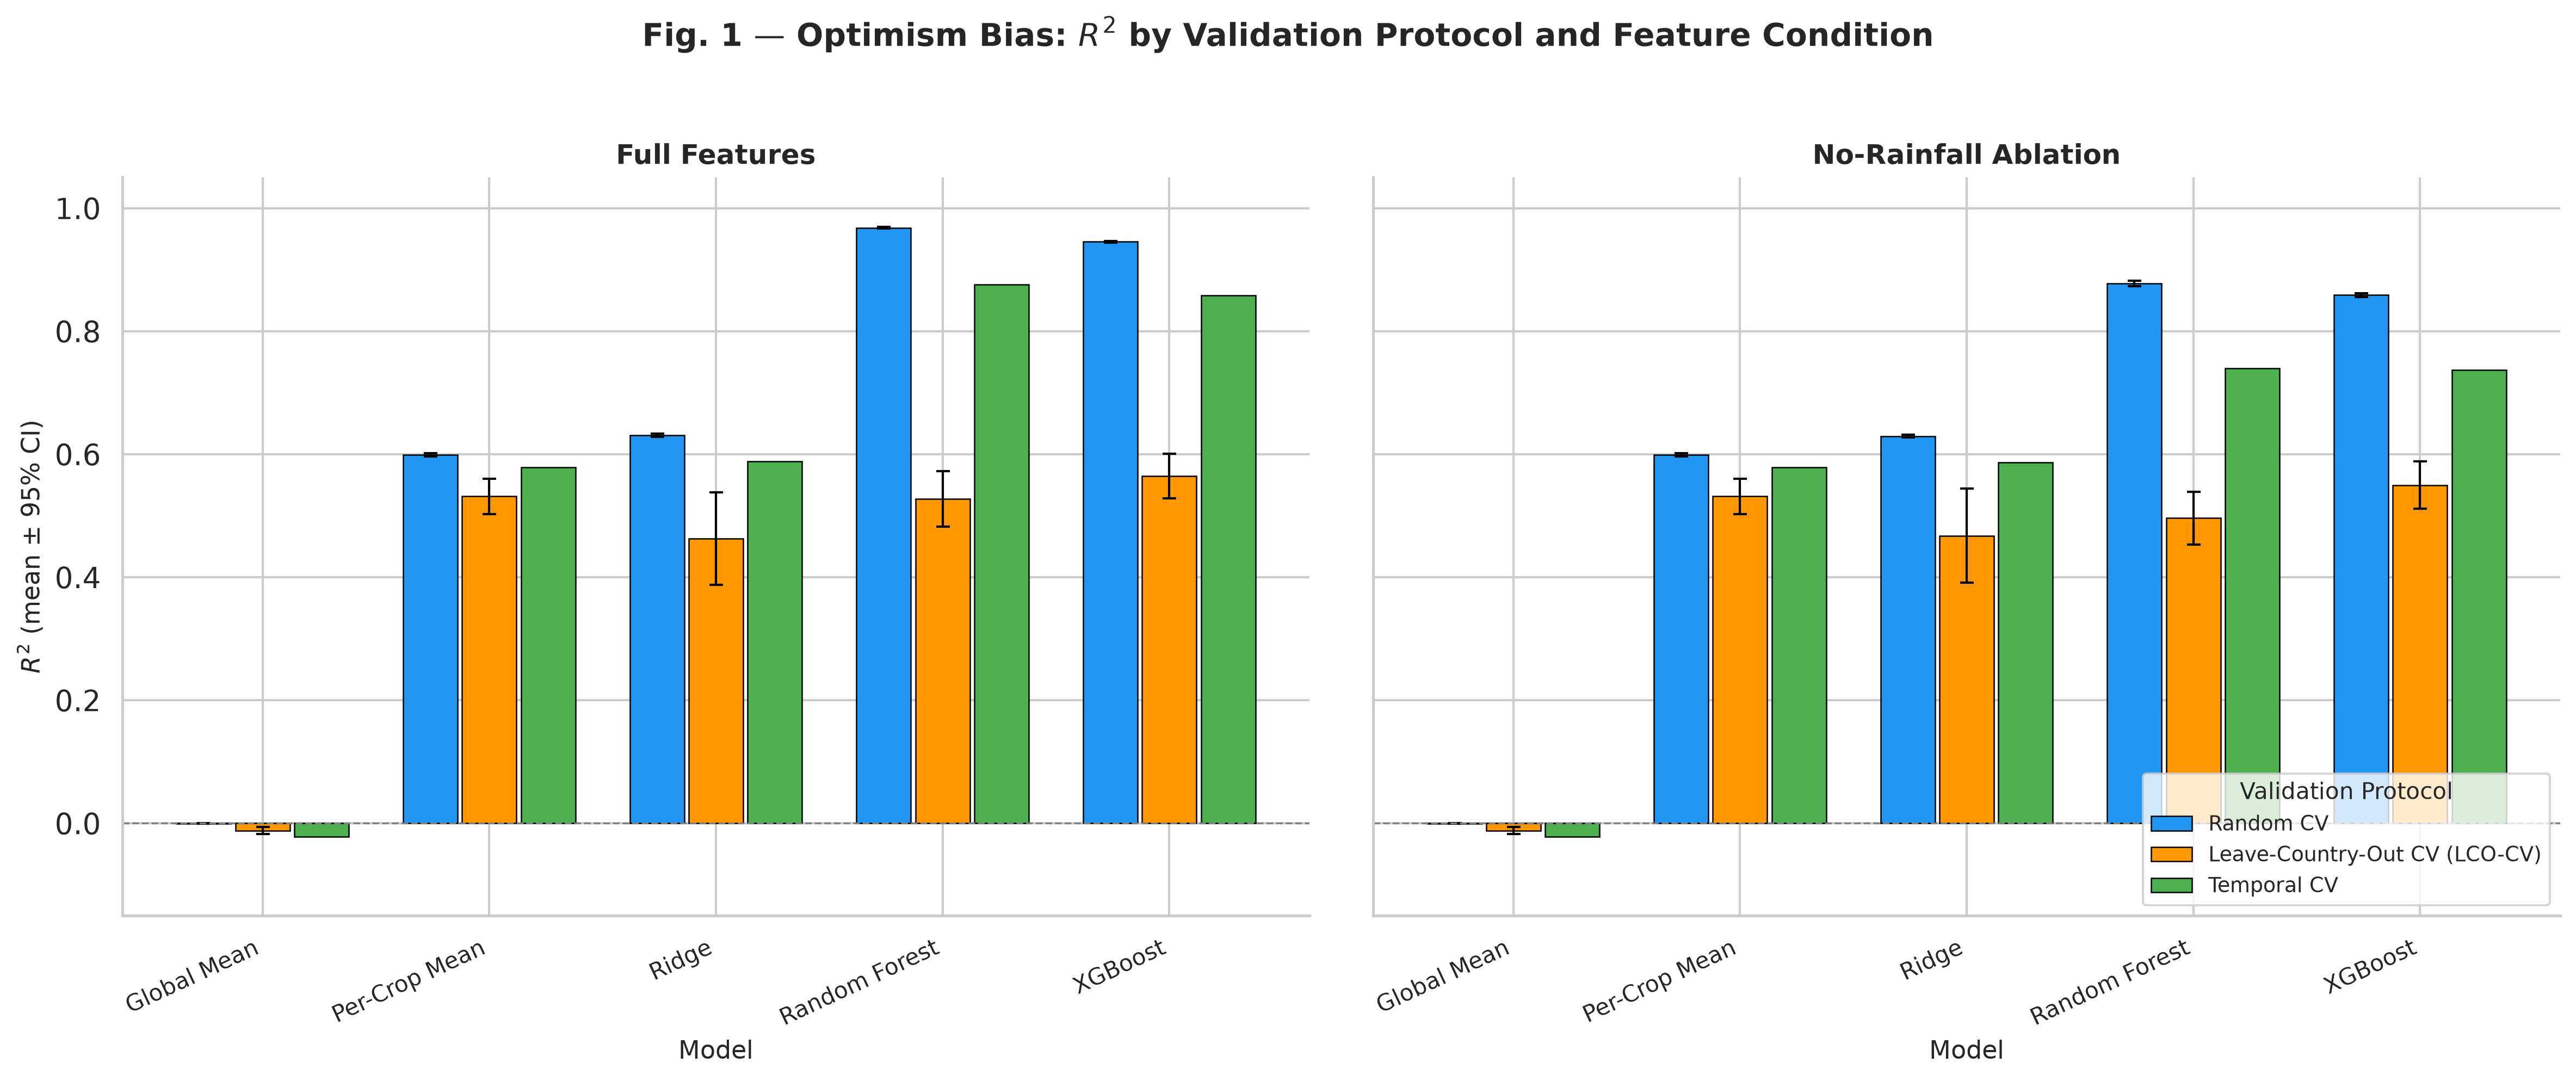
\includegraphics[width=\textwidth]{fig1_protocol_ablation.png}
  \caption{$R^2$ (mean $\pm$ approximate 95\% CI) across validation protocols 
           under Full Features (left) and No-Rainfall Ablation (right). Error bars 
           reflect 20 repeated splits for Random CV and LCO-CV (omitted for Temporal CV, 
           which plots deterministic cutoff point-estimate means). The performance 
           collapse of tree ensembles under LCO-CV highlights the optimism gap.}
  \label{fig:protocol_ablation}
\end{figure*}

The optimism gap\footnote{The mean of per-fold differences ($0.441 \pm 0.104$ for RF, 
$0.381 \pm 0.084$ for XGB) differs by $\leq 0.001$ from the difference of protocol 
means ($0.968 - 0.528 = 0.440$ for RF, $0.945 - 0.564 = 0.381$ for XGB) due to rounding.} 
is \textbf{0.44 points for Random Forest} and \textbf{0.38 points for XGBoost}. 
Under LCO-CV, high fold-to-fold variance ($\text{SD} \approx 0.08\text{--}0.10$) 
means RF (0.528) and XGBoost (0.564) are not statistically distinguishable from each other.

Crucially, under LCO-CV, Random Forest ($R^2 = 0.528 \pm 0.103$) shows 
\textbf{no detectable difference from the naive Per-Crop Mean baseline} 
($R^2 = 0.531 \pm 0.065$). The paired per-split difference between Random Forest 
and Per-Crop Mean under LCO-CV is $\Delta = -0.004 \pm 0.099$ (approximate 95\% CI: 
$[-0.050, 0.042]$, $p = 0.87$). XGBoost ($0.564 \pm 0.083$) achieves only a 
marginal, practically negligible improvement ($\Delta = +0.033 \pm 0.062$, 95\% CI: 
$[0.004, 0.062]$). Because the 20 splits overlap, standard $p$-values and intervals 
are optimistic, so this modest shift must be interpreted cautiously. A complex tree 
ensemble offers essentially no proven advantage on unseen countries over a simple 
lookup table of average crop yields.

\subsection{Ablation and Feature Importance}

Table~\ref{tab:r2_ablation} shows results after removing \texttt{average\_rain\_fall\_mm\_per\_year}.

\begin{table}[t]
\centering
\caption{$R^2$ by Model and Protocol (No-Rainfall Ablation, mean $\pm$ SD)}
\label{tab:r2_ablation}
\resizebox{\columnwidth}{!}{%
\begin{tabular}{lccc}
\toprule
\textbf{Model} & \textbf{Random CV} & \textbf{LCO-CV} & \textbf{Temporal CV}\textsuperscript{*} \\
\midrule
Global Mean     & $-0.000\pm0.000$ & $-0.012\pm0.013$ & $-0.022$ \\
Per-Crop Mean   & $0.599\pm0.006$  & $0.531\pm0.065$  & $0.578$  \\
Ridge           & $0.629\pm0.005$  & $0.468\pm0.175$  & $0.587$  \\
Random Forest   & $0.878\pm0.010$  & $0.496\pm0.098$  & $0.740$  \\
XGBoost         & $0.859\pm0.007$  & $0.550\pm0.087$  & $0.737$  \\
\bottomrule
\multicolumn{4}{l}{\footnotesize\textsuperscript{*}Point-estimate mean across the five forward temporal cutoffs.}
\end{tabular}%
}
\end{table}

Under Random CV, removing rainfall produces an immediate drop of 
$\Delta = -0.091 \pm 0.009$ for RF and $-0.087 \pm 0.005$ for XGBoost ($p < 0.001$). 
In contrast, under LCO-CV, the changes (RF: $-0.032 \pm 0.091$; XGB: $-0.014 \pm 0.075$) 
are statistically indistinguishable from zero, indicating that rainfall conveyed no 
detectable geographic generalisation signal.

Because the 20 splits share identical random seeds across Full and Ablation runs, 
we compute the paired gap reduction\footnote{The ratio of means yields 
$0.059 / 0.441 \approx 13.4\%$ for RF and $0.072 / 0.381 \approx 18.9\%$ for XGBoost. 
The mean of per-split percentage reductions is $11.6\%$ for RF and $17.9\%$ for XGBoost. 
Per-split values span a broad range ($-48\%$ to $+35\%$ for RF, $-10\%$ to $+45\%$ 
for XGBoost) due to high LCO-CV fold variance. The gap reduction is real on average 
but not uniform across individual splits.}. For Random Forest, the gap decreases by 
$0.059 \pm 0.089$ (approximate 95\% CI: $[0.018, 0.101]$). For XGBoost, the gap 
decreases by $0.072 \pm 0.075$ (approximate 95\% CI: $[0.037, 0.107]$). 
While the Random CV drop is tight, the high variance of LCO-CV introduces 
noticeable dispersion into the estimated net reduction.

To assess how models utilise continuous features under Random CV, 
Table~\ref{tab:importances} reports both Mean Decrease in Impurity (MDI) 
and Permutation Importance on held-out test splits.

\begin{table}[t]
\centering
\caption{Feature Importance under Random CV (mean $\pm$ SD over splits)}
\label{tab:importances}
\resizebox{\columnwidth}{!}{%
\begin{tabular}{lcccc}
\toprule
\multirow{2}{*}{\textbf{Feature}} 
  & \multicolumn{2}{c}{\textbf{Random Forest}} 
  & \multicolumn{2}{c}{\textbf{XGBoost}} \\
  \cmidrule(lr){2-3}\cmidrule(lr){4-5}
  & MDI (\%) & Perm ($\Delta R^2$) & MDI (\%) & Perm ($\Delta R^2$) \\
\midrule
\texttt{avg\_rain\_mm}      & $11.9\pm0.2$ & $\mathbf{0.370\pm0.011}$ & $1.6\pm0.1$ & $\mathbf{0.279\pm0.011}$ \\
\texttt{pesticides\_tonnes} & $15.1\pm0.5$ & $0.329\pm0.013$ & $1.6\pm0.1$ & $0.229\pm0.013$ \\
\texttt{avg\_temp}          & $12.8\pm0.6$ & $0.293\pm0.013$ & $2.1\pm0.2$ & $0.225\pm0.013$ \\
\texttt{Item\_Potatoes}     & $37.1\pm0.2$ & $1.125\pm0.019$ & $44.1\pm3.8$ & $1.007\pm0.017$ \\
\texttt{Item\_Cassava}      & $9.2\pm0.1$  & $0.335\pm0.007$ & $22.3\pm3.1$ & $0.279\pm0.007$ \\
\texttt{Item\_Sweet pot}    & $8.5\pm0.1$  & $0.296\pm0.017$ & $9.6\pm0.6$  & $0.214\pm0.012$ \\
\bottomrule
\end{tabular}%
}
\end{table}

While MDI can overstate high-cardinality continuous features, and permutation 
importance can be influenced by collinearity, held-out permutation tests indicate 
that \texttt{avg\_rain\_mm} is among the most influential continuous features 
($\Delta R^2 = 0.370 \pm 0.011$ in RF, $0.279 \pm 0.011$ in XGBoost), slightly 
exceeding pesticide tonnage ($0.329 / 0.229$) and temperature ($0.293 / 0.225$). 
Tree models likely exploit rainfall thresholds to partition data into country clusters, 
while correlated pesticide and temperature distributions provide complementary 
fingerprint signals.

\subsection{Error Magnitude and Disaggregation}

Table~\ref{tab:full_metrics} presents MAE and RMSE for the Full feature condition.

\begin{table}[t]
\centering
\caption{MAE and RMSE (hg/ha) by Model and Protocol (Full Features, mean $\pm$ SD)}
\label{tab:full_metrics}
\resizebox{\columnwidth}{!}{%
\begin{tabular}{lcccc}
\toprule
\multirow{2}{*}{\textbf{Model}} 
  & \multicolumn{2}{c}{\textbf{Random CV}} 
  & \multicolumn{2}{c}{\textbf{LCO-CV}} \\
  \cmidrule(lr){2-3}\cmidrule(lr){4-5}
  & MAE & RMSE & MAE & RMSE \\
\midrule
Global Mean   & $63{,}723\pm604$   & $84{,}479\pm1236$  & $64{,}953\pm3714$ & $87{,}590\pm8430$ \\
Per-Crop Mean & $33{,}331\pm506$   & $53{,}463\pm904$   & $36{,}858\pm4558$ & $59{,}454\pm6747$ \\
Ridge         & $32{,}190\pm499$   & $51{,}322\pm860$   & $40{,}503\pm6955$ & $62{,}766\pm7758$ \\
Random Forest & $6{,}441\pm208$    & $15{,}045\pm714$   & $35{,}836\pm4218$ & $59{,}278\pm6183$ \\
XGBoost       & $11{,}667\pm236$   & $19{,}737\pm612$   & $34{,}314\pm4494$ & $57{,}100\pm6677$ \\
\bottomrule
\end{tabular}%
}
\end{table}

Random Forest MAE degrades from 6{,}441~hg/ha under Random CV to 35{,}836~hg/ha 
under LCO-CV (a 5.6$\times$ increase). Figure~\ref{fig:error_by_crop} disaggregates 
errors by crop for XGBoost: the inflation is universal across crops, though absolute 
error magnitudes vary by species (Cassava and Yams show wider spreads due to larger 
inherent yield variability).

\subsection{Forward Temporal Evaluation}

Table~\ref{tab:temporal} and Figure~\ref{fig:temporal_drift} show performance 
across expanding temporal training horizons.

\begin{table}[t]
\centering
\caption{RMSE (hg/ha) by Model and Temporal Cutoff (Full Features, point estimates)}
\label{tab:temporal}
\resizebox{\columnwidth}{!}{%
\begin{tabular}{lccccc}
\toprule
\textbf{Model} & \textbf{2002} & \textbf{2004} & \textbf{2006} & \textbf{2008} & \textbf{2010} \\
\midrule
Global Mean   & 93{,}089 & 93{,}394 & 94{,}802 & 95{,}830 & 97{,}116 \\
Per-Crop Mean & 60{,}138 & 60{,}154 & 60{,}985 & 61{,}344 & 61{,}967 \\
Ridge         & 60{,}286 & 59{,}888 & 60{,}222 & 60{,}057 & 60{,}354 \\
Random Forest & 37{,}397 & 33{,}519 & 34{,}080 & 28{,}845 & 30{,}311 \\
XGBoost       & 39{,}514 & 35{,}555 & 36{,}663 & 31{,}451 & 32{,}261 \\
\bottomrule
\end{tabular}%
}
\end{table}

Tree ensembles achieve lower RMSE as training data accumulates (2002 to 2008 cutoffs), 
yielding higher nominal test $R^2$ than under LCO-CV. However, as discussed below, 
temporal splits retain identical countries across train and test partitions, so 
country-identity leakage remains operational during temporal evaluation.

\begin{figure*}[t]
  \centering
  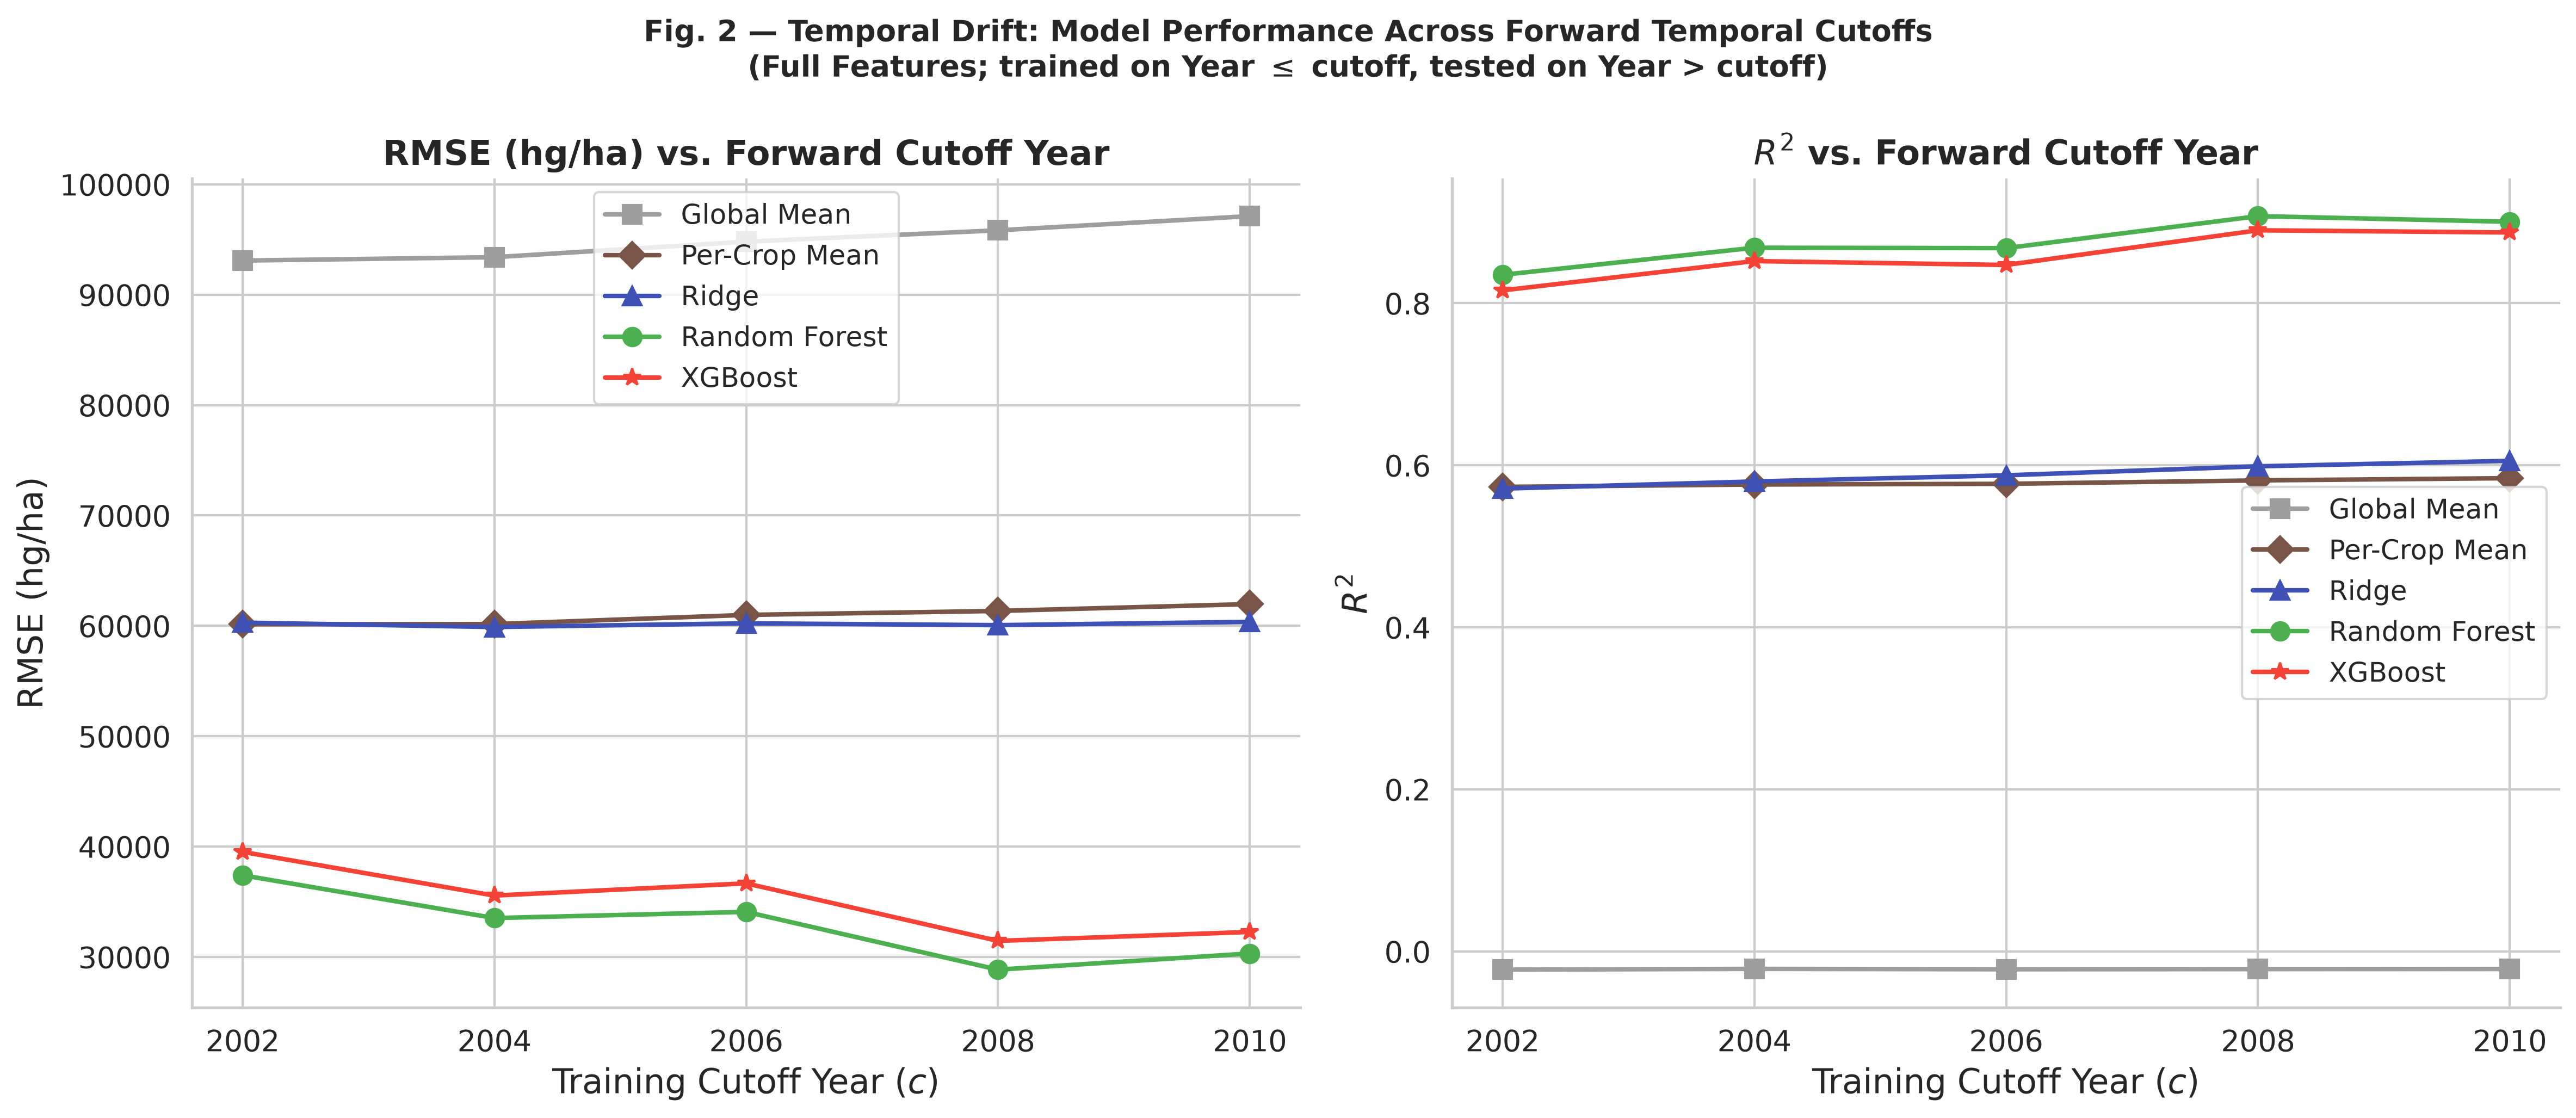
\includegraphics[width=0.92\textwidth]{fig2_temporal_drift.png}
  \caption{RMSE (left) and $R^2$ (right) across forward temporal cutoffs 
           (Full Features; confounded by persistent country identity across splits). 
           Tree ensembles improve as training horizons grow, while linear models 
           remain static.}
  \label{fig:temporal_drift}
\end{figure*}

\begin{figure*}[t]
  \centering
  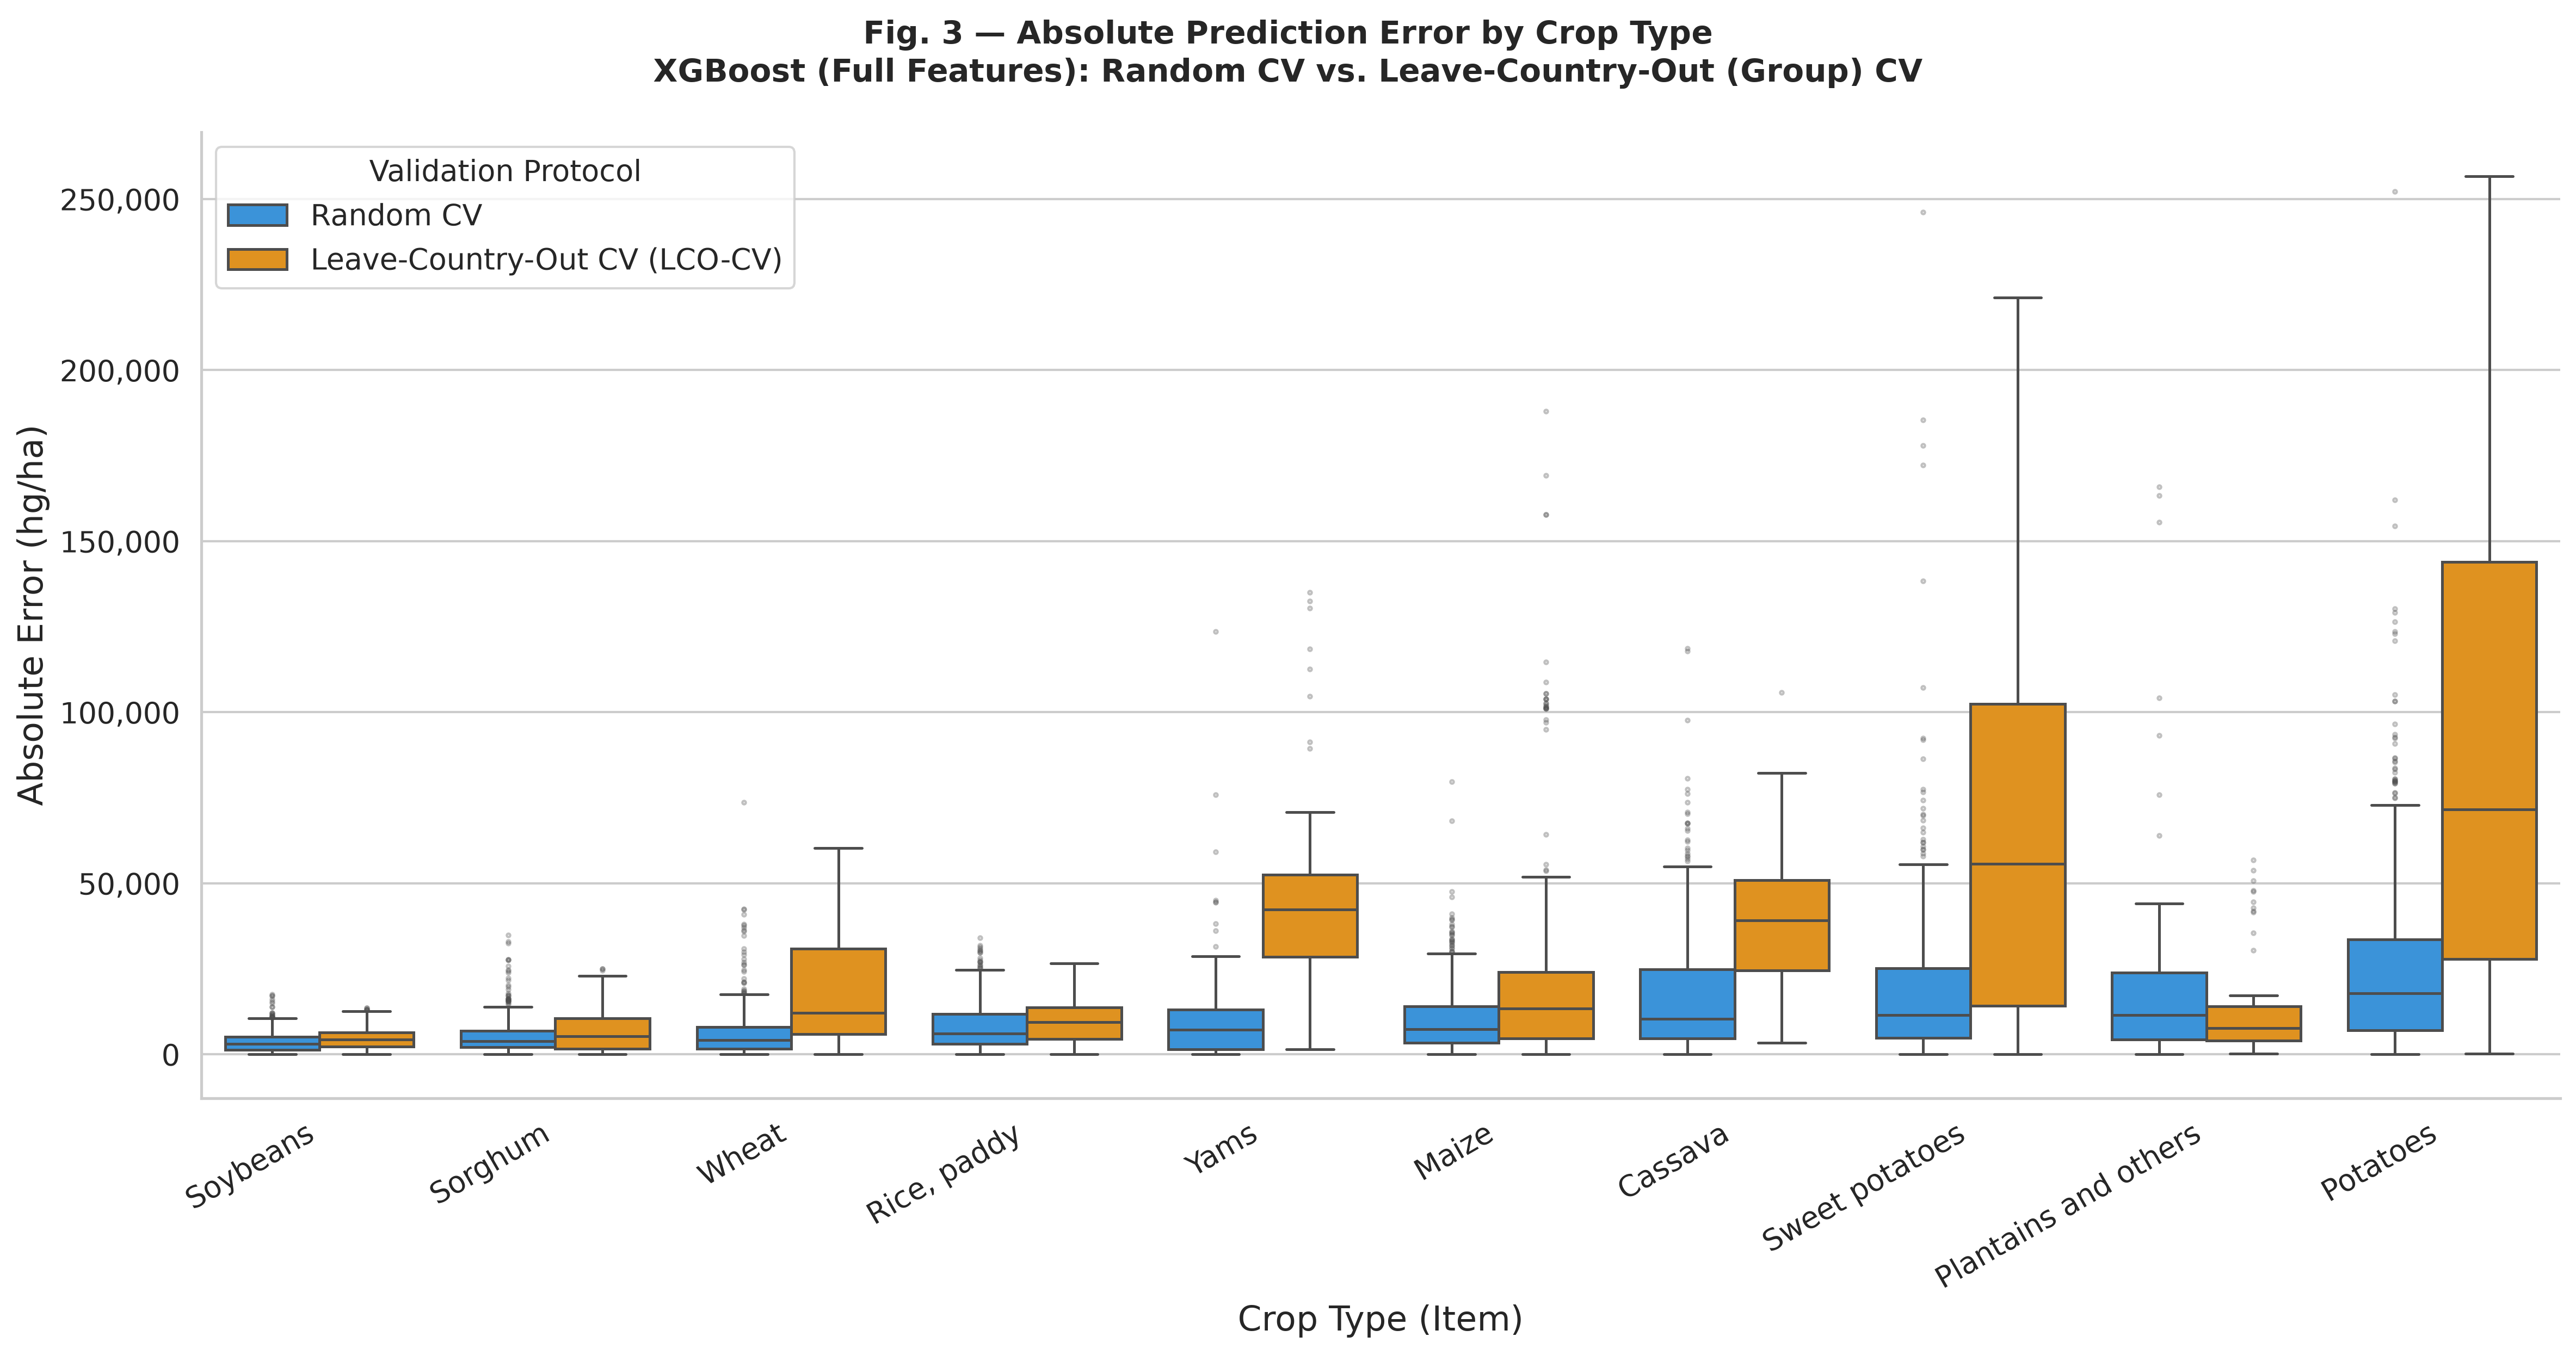
\includegraphics[width=0.92\textwidth]{fig3_error_by_crop.png}
  \caption{Absolute prediction error (hg/ha) by crop type for XGBoost 
           under Random CV vs.\ Leave-Country-Out CV (LCO-CV). The gap 
           is consistent in direction across all 10 crop species.}
  \label{fig:error_by_crop}
\end{figure*}

%% ============================================================
\section{Discussion}
\label{sec:discussion}

\subsection{Magnitude of Optimism Bias}

The 0.38--0.44 $R^2$ optimism gap observed here is in the same direction as the 
performance collapse reported by Ploton et al.~\cite{ploton2020} in ecological 
mapping (where spatial validation reduced apparent predictive skill to quasi-null 
levels), though in our benchmark tree models collapse to the crop-mean baseline 
rather than zero. In agricultural prediction, optimism is plausibly amplified 
because tabular datasets often aggregate observations into country-level administrative 
units where environmental features correlate strongly with geographic boundaries.

\subsection{The Proxy Leakage Mechanism}

Ablation isolates the impact of the time-invariant rainfall proxy, reducing the 
paired optimism gap by roughly 13--19\% on average ($0.059$ to $0.072$ $R^2$ points). 
The residual gap (${\approx}0.31$--$0.38$) is consistent with spatial 
autocorrelation and/or country memorisation via other covariates (such as 
distinct country-level distributions of pesticides and temperature). Replacing 
rainfall with dynamic time-varying measurements would likely not eliminate this 
gap, as country-level agricultural clustering would persist.

\subsection{The Per-Crop Mean Baseline Floor}

Under Leave-Country-Out CV, Random Forest ($R^2 = 0.528$) shows no detectable 
difference from predicting each crop's historical average ($R^2 = 0.531$). Despite 
achieving near-perfect training and Random CV scores ($R^2 = 0.95$--$0.97$), complex 
tree ensembles demonstrate negligible geographic transferability on this dataset. 
Establishing naive baselines is essential to diagnose whether ML models learn 
generalisable agronomic relationships or merely memorise local identities.

\subsection{Limitations}
\label{sec:limitations}

\begin{itemize}
    \item \textbf{Random group splits}: LCO-CV randomly allocates countries rather 
    than enforcing spatial buffer zones; neighbouring countries may still share boundaries.
    
    \item \textbf{Temporal CV confound}: The same countries appear in both train and test 
    folds in Protocol C, so country-identity leakage remains active.
    
    \item \textbf{Overlapping splits}: The 20 repeated splits overlap, making $t$-distribution 
    confidence intervals approximate.
    
    \item \textbf{National aggregate pesticide feature}: The \texttt{pesticides\_tonnes} 
    feature represents national total consumption rather than application intensity per hectare. 
    It consequently correlates with country size rather than agronomic practices, which may 
    partly explain why tree models add little value under LCO-CV; this outcome could reflect 
    uninformative input covariates rather than inherent limitations of the model architectures.
    
    \item \textbf{Split-to-split gap reduction variance}: While rainfall ablation reduces 
    the optimism gap by 13--19\% on average, the per-split reduction varies between $-48\%$ 
    and $+35\%$ for RF (and $-10\%$ to $+45\%$ for XGBoost), indicating that the leakage 
    penalty is real on average but not uniform across individual geographic partitions.
    
    \item \textbf{Hyperparameters}: Models use default hyperparameters; systematic tuning 
    could alter gap magnitudes.
    
    \item \textbf{Mechanistic identification}: While permutation importance indicates heavy 
    reliance on rainfall alongside pesticides and temperature, country memorisation remains 
    an inferred mechanism without explicit country one-hot ablation.
\end{itemize}

%% ============================================================
\section{Conclusion}
\label{sec:conclusion}

Standard random cross-validation inflates reported $R^2$ by 0.38--0.44 points 
for tree ensembles on this crop yield benchmark. Under Leave-Country-Out CV, 
Random Forest shows no detectable difference from a naive Per-Crop Mean baseline. 
A data audit and ablation indicate that time-invariant rainfall proxy leakage explains 
roughly 13--19\% of this inflation on average, with permutation tests indicating that 
models rely on rainfall alongside pesticides and temperature as geographic identifiers 
under random splits. Structure-aware validation protocols and naive domain baselines 
must become standard practice in applied agricultural ML.

%% ============================================================
\section*{Acknowledgements}
The author thanks the FAO and the World Bank for making the underlying agricultural 
data publicly accessible.

%% ============================================================
\bibliographystyle{IEEEtran}
\bibliography{references}

\end{document}
